\chapter\bigskip
\ifpdf
  \graphicspath{{AppendixA/AppendixAFigs/PNG/}{AppendixA/AppendixAFigs/PDF/}{AppendixA/AppendixAFigs/}}
\else
  \graphicspath{{AppendixA/AppendixAFigs/EPS/}{AppendixA/AppendixAFigs/}}
\fi
% \setboolean{@twoside}{false}
% doublepages
\section{Manual de Usuario de \textit{TapeYty}}
\label{sec:manual-usuario}
\includepdf[pages=-, pagecommand={}, nup=1x2, width=\textwidth, offset=32mm -5mm]{AppendixA/AppendixPdf/Manual_de_usuario.pdf}
% \begin{figure}[H]
%     \begin{center}
%         \subfigure[][\label{fig:img1} $SSIM = 1$ \newline $LTG = 1 $ \newline $\mathscr{H} = 7.4428$ \newline $\mathscr E =3.4754$]
%         {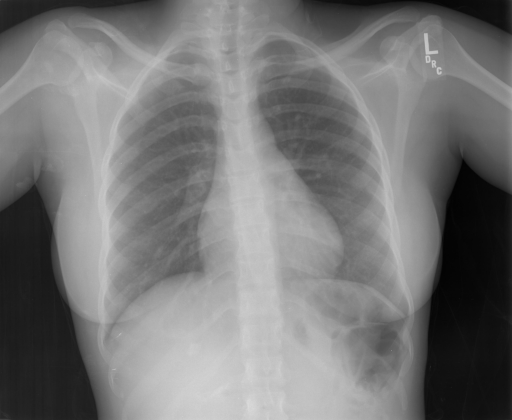
\includegraphics[width=4.5cm]{AppendixA/AppendixAFigs/originales/frontales/imagen1.png}}
%         \subfigure[][\label{fig:img2} $SSIM = 1$ \newline $LTG = 1$ \newline $\mathscr{H} = 6.6690$ \newline $\mathscr E =2.9755$
%         ]{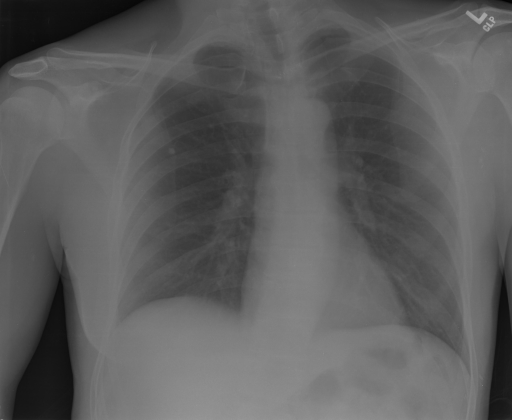
\includegraphics[width=4.5cm]{AppendixA/AppendixAFigs/originales/frontales/imagen2.png}}
%         \subfigure[][\label{fig:img4} $SSIM = 1$ \newline $LTG = 1$ \newline $\mathscr{H} = 7.1196$ \newline $\mathscr E =3.4570$
%         ]{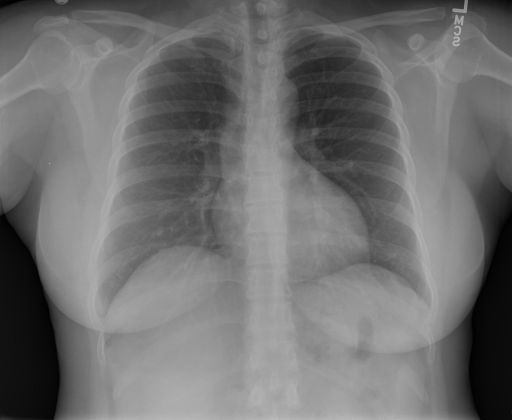
\includegraphics[width=4.5cm]{AppendixA/AppendixAFigs/originales/frontales/imagen4.png}}
%     \end{center}
%     \label{fig:gral1}
% \end{figure}

% \begin{figure}[H]
%     \begin{center}
%         \subfigure[][\label{fig:img3} $SSIM = 1$ \newline $LTG = 1$ \newline $\mathscr{H} = 7.3003$ \newline $\mathscr E =3.7876$
%         ]{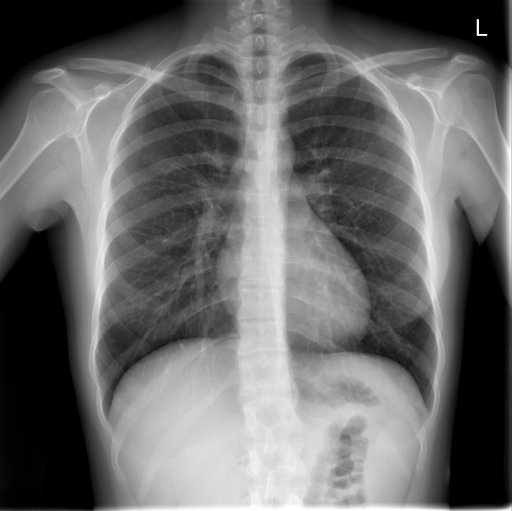
\includegraphics[width=4.5cm]{AppendixA/AppendixAFigs/originales/frontales/imagen3.png}}
%         \subfigure[][\label{fig:img5} $SSIM = 1$ \newline $LTG = 1$ \newline $\mathscr{H} = 7.4409$ \newline $\mathscr E =3.5873$
%         ]{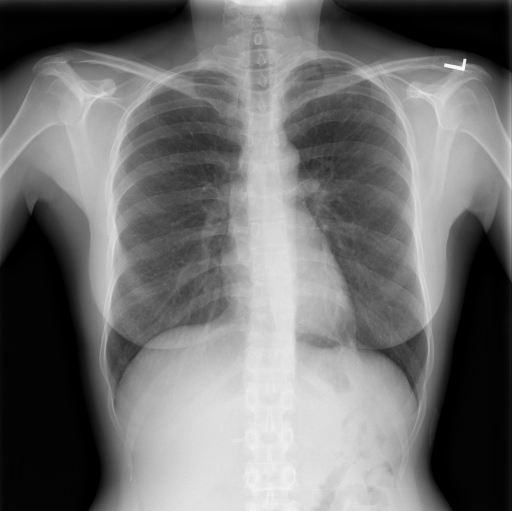
\includegraphics[width=4.5cm]{AppendixA/AppendixAFigs/originales/frontales/imagen5.png}}
%         \subfigure[][\label{fig:img7} $SSIM = 1$ \newline $LTG = 1$ \newline $\mathscr{H} = 7.7184$ \newline $\mathscr E =3.9015$
%         ]{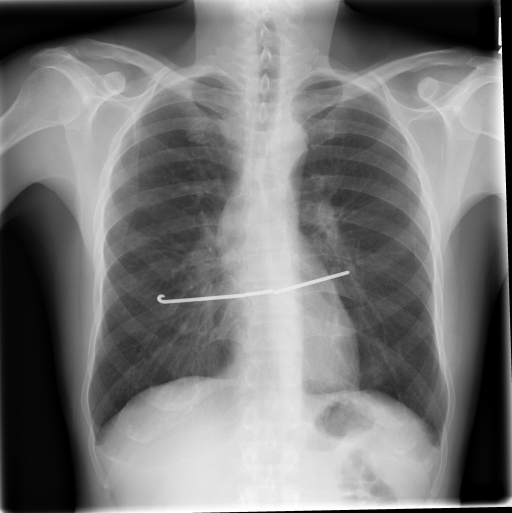
\includegraphics[width=4.5cm]{AppendixA/AppendixAFigs/originales/frontales/imagen7.png}}
%     \end{center}
%     \label{fig:gral2}
% \end{figure}

% \begin{figure}[H]
%     \begin{center}
%         \subfigure[][\label{fig:img6}  $SSIM = 1$ \newline $LTG = 1$ \newline $\mathscr{H} = 6.8287$ \newline $\mathscr E =3.1996$
%         ]{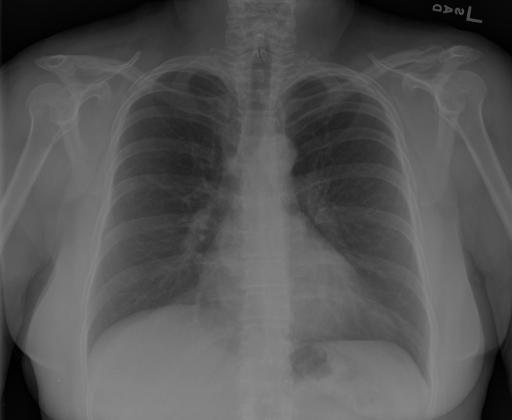
\includegraphics[width=4.5cm]{AppendixA/AppendixAFigs/originales/frontales/imagen6.png}}
%         \subfigure[][\label{fig:img8}  $SSIM = 1$ \newline $LTG = 1$ \newline $\mathscr{H} = 6.8998$ \newline $\mathscr E =3.3196$
%         ]{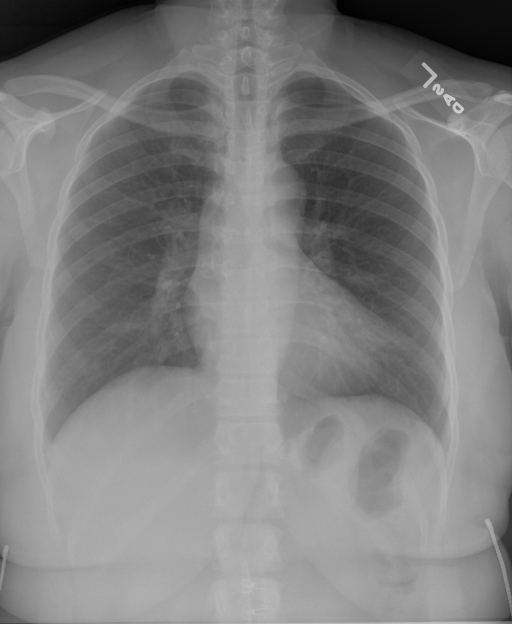
\includegraphics[width=3.0cm]{AppendixA/AppendixAFigs/originales/frontales/imagen8.png}}
%         \subfigure[][\label{fig:img9}  $SSIM = 1$ \newline $LTG =1 $ \newline $\mathscr{H} = 6.6672$ \newline $\mathscr E =3.4084$
%         ]{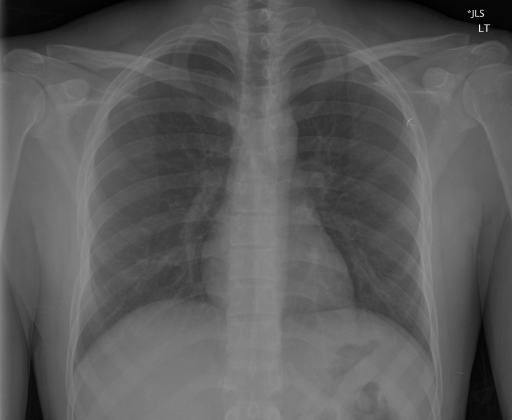
\includegraphics[width=4.5cm]{AppendixA/AppendixAFigs/originales/frontales/imagen9.png}}
%     \end{center}
%     \label{fig:gral3}
% \end{figure}

% \begin{figure}[H]
%     \begin{center}
%         \subfigure[][\label{fig:img10}  $SSIM = 1$ \newline $LTG = 1$ \newline $\mathscr{H} = 6.8803$ \newline $\mathscr E =3.3658$
%         ]{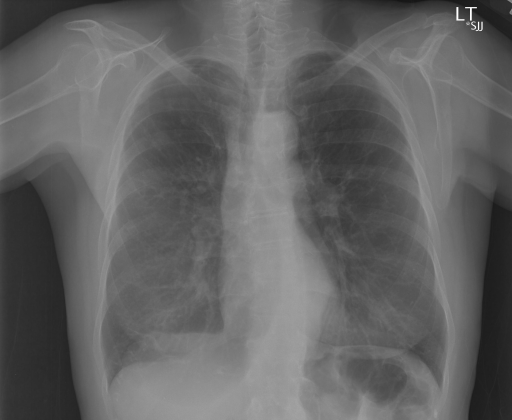
\includegraphics[width=4.5cm]{AppendixA/AppendixAFigs/originales/frontales/imagen10.png}}
%         \subfigure[][\label{fig:img11}  $SSIM = 1$ \newline $LTG = 1$ \newline $\mathscr{H} = 7.5582$ \newline $\mathscr E =3.5560$
%         ]{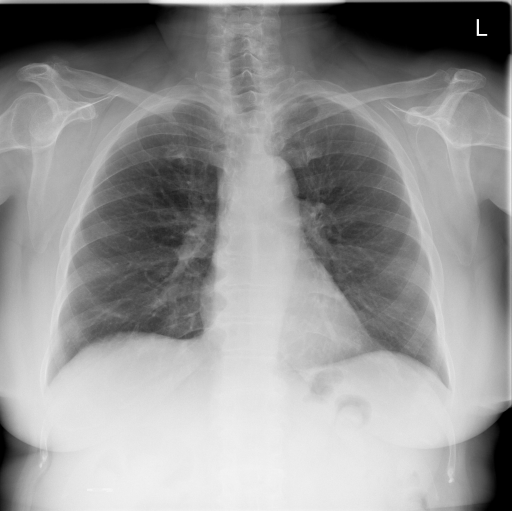
\includegraphics[width=3.7cm]{AppendixA/AppendixAFigs/originales/frontales/imagen11.png}}
%         \subfigure[][\label{fig:img12}  $SSIM = 1$ \newline $LTG = 1$ \newline $\mathscr{H} = 6.5775$ \newline $\mathscr E =3.02324.1202$
%         ]{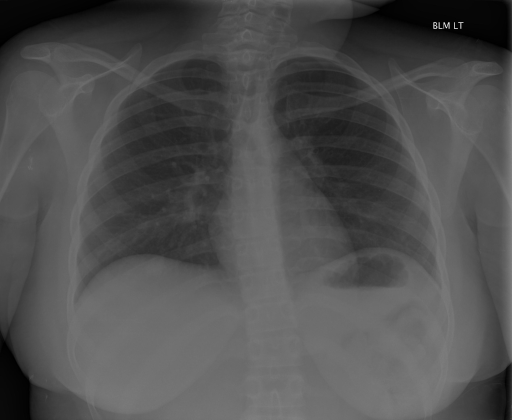
\includegraphics[width=4.5cm]{AppendixA/AppendixAFigs/originales/frontales/imagen12.png}}
%     \end{center}
%     \label{fig:gral4}
% \end{figure}

% \begin{figure}[H]
%     \begin{center}
%         \subfigure[][\label{fig:img13}  $SSIM = 1$ \newline $LTG = 1$ \newline $\mathscr{H} = 7.5991$ \newline $\mathscr E =4.1202$
%         ]{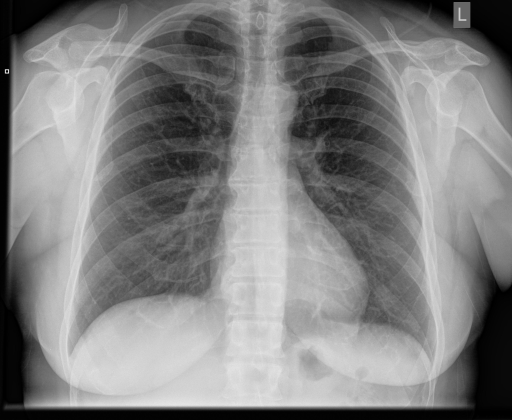
\includegraphics[width=4.5cm]{AppendixA/AppendixAFigs/originales/frontales/imagen13.png}}
%         \subfigure[][\label{fig:img14}  $SSIM = 1$ \newline $LTG = 1$ \newline $\mathscr{H} = 6.9048$ \newline $\mathscr E =3.4270$
%         ]{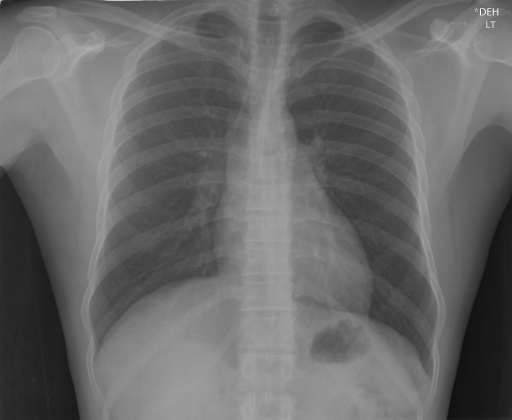
\includegraphics[width=4.5cm]{AppendixA/AppendixAFigs/originales/frontales/imagen14.png}}
%         \subfigure[][\label{fig:img15}  $SSIM = 1$ \newline $LTG = 1$ \newline $\mathscr{H} = 6.7262$ \newline $\mathscr E =3.1108$
%         ]{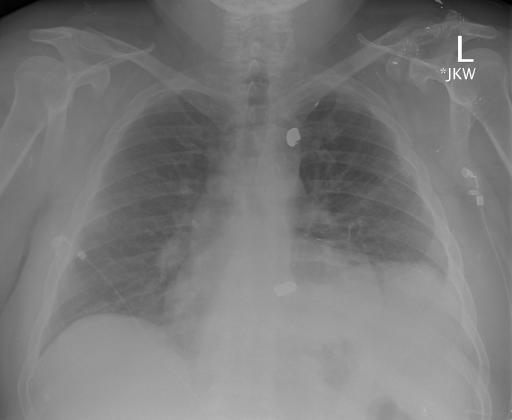
\includegraphics[width=4.5cm]{AppendixA/AppendixAFigs/originales/frontales/imagen15.png}}
%     \end{center}
%     \label{fig:gral5}
% \end{figure}


% \begin{figure}[H]
%     \begin{center}
%         \subfigure[][\label{fig:imgtll} $SSIM = 1$ \newline $LTG = 1 $ \newline $\mathscr{H} = 7.2447$ \newline $\mathscr E = 2.8626$]
%         {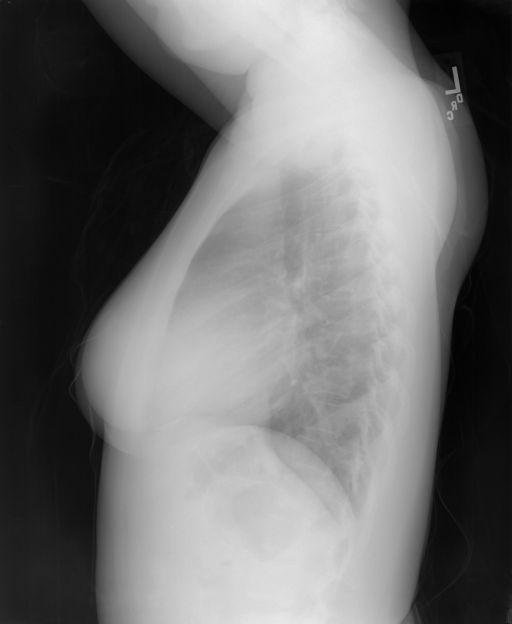
\includegraphics[width=4cm]{AppendixA/AppendixAFigs/originales/laterales/imagen1.png}}
%         \subfigure[][\label{fig:imgtl2} $SSIM = 1$ \newline $LTG = 1$ \newline $\mathscr{H} =7.1010 $ \newline $\mathscr E = 2.8157$
%         ]{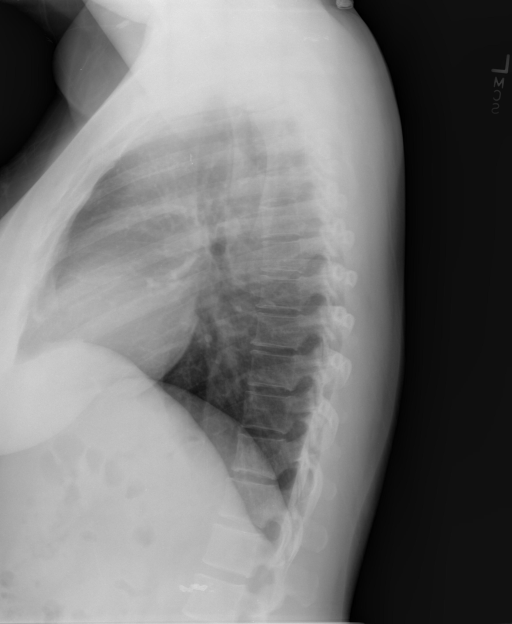
\includegraphics[width=4cm]{AppendixA/AppendixAFigs/originales/laterales/imagen2.png}}
%         \subfigure[][\label{fig:imgtl4} $SSIM = 1$ \newline $LTG = 1 $ \newline $\mathscr{H} = 6.7004$ \newline $\mathscr E = 2.7408$]
%         {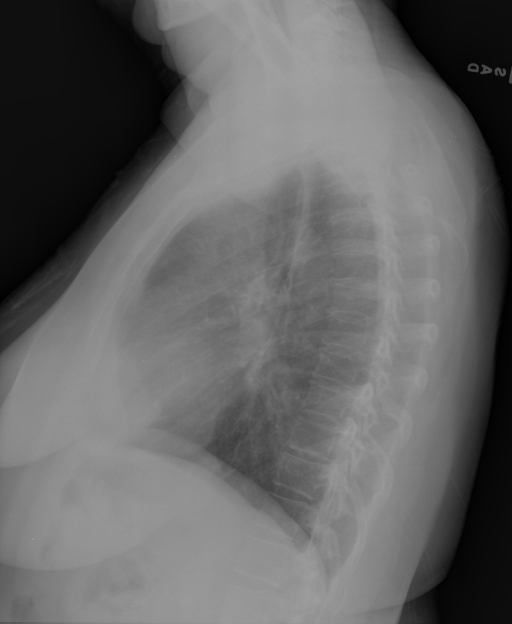
\includegraphics[width=4cm]{AppendixA/AppendixAFigs/originales/laterales/imagen4.png}}
%     \end{center}
%     \label{fig:gral6}
% \end{figure}

% \begin{figure}[H]
%     \begin{center}
       
%         \subfigure[][\label{fig:imgtl6} $SSIM = 1$ \newline $LTG = 1$ \newline $\mathscr{H} = 5.8141$ \newline $\mathscr E = 1.9030$
%         ]{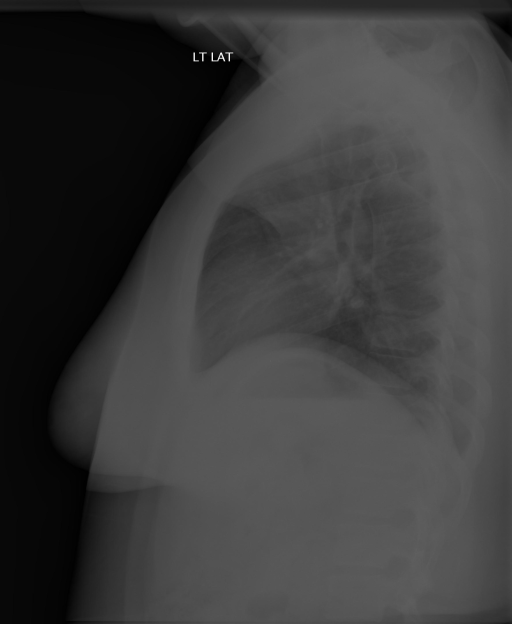
\includegraphics[width=4cm]{AppendixA/AppendixAFigs/originales/laterales/imagen6.png}}
%       \subfigure[][\label{fig:imgtl7} $SSIM = 1$ \newline $LTG = 1 $ \newline $\mathscr{H} = 6.9070$ \newline $\mathscr E = 2.9594$]
%         {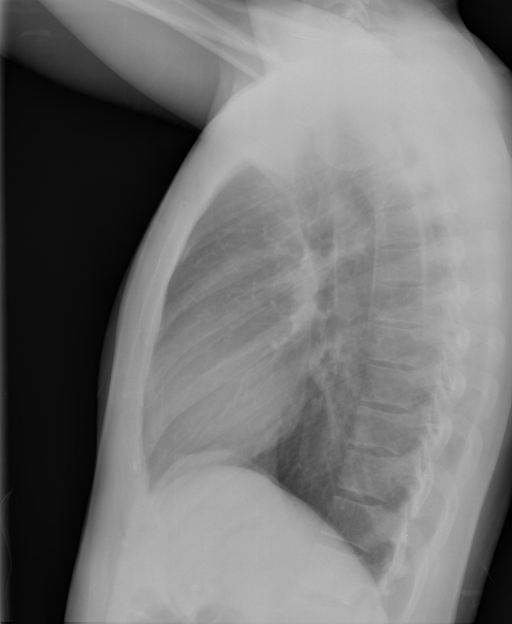
\includegraphics[width=4cm]{AppendixA/AppendixAFigs/originales/laterales/imagen7.png}}
%         \subfigure[][\label{fig:imgtl8} $SSIM = 1$ \newline $LTG = 1$ \newline $\mathscr{H} = 7.0622$ \newline $\mathscr E = 2.9446$
%         ]{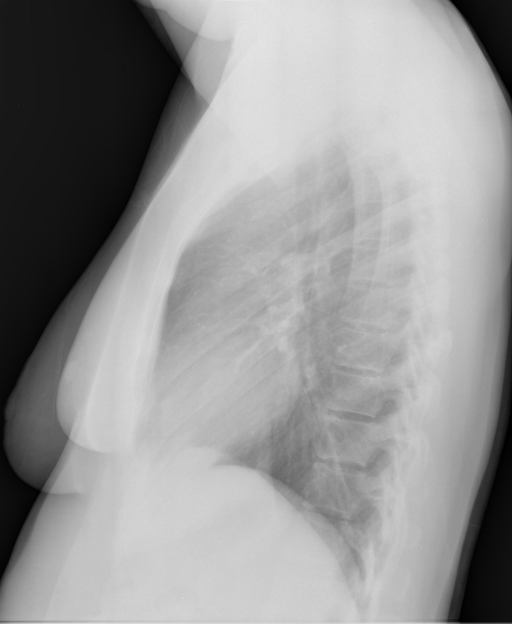
\includegraphics[width=4cm]{AppendixA/AppendixAFigs/originales/laterales/imagen8.png}}
%     \end{center}
%     \label{fig:gral7}
% \end{figure}

% \begin{figure}[H]
%     \begin{center}
        
%         \subfigure[][\label{fig:imgtl9} $SSIM = 1$ \newline $LTG = 1$ \newline $\mathscr{H} = 7.5625$ \newline $\mathscr E = 3.4395$
%         ]{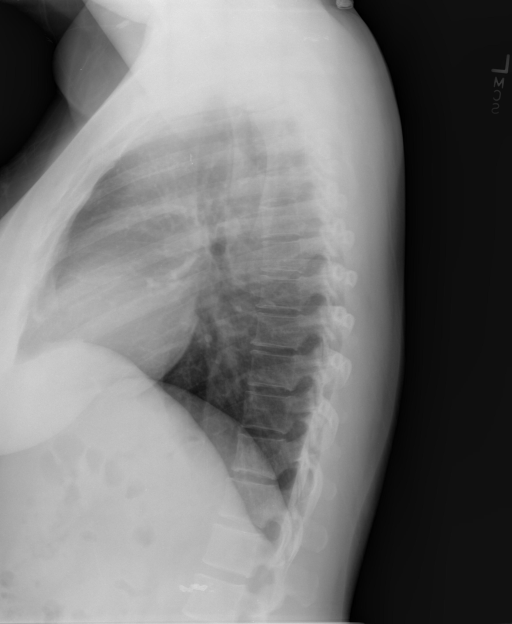
\includegraphics[width=4cm]{AppendixA/AppendixAFigs/originales/laterales/imagen9.png}}
%         \subfigure[][\label{fig:imgtl10} $SSIM = 1$ \newline $LTG = 1 $ \newline $\mathscr{H} = 7.1064$ \newline $\mathscr E = 3.3058$]
%         {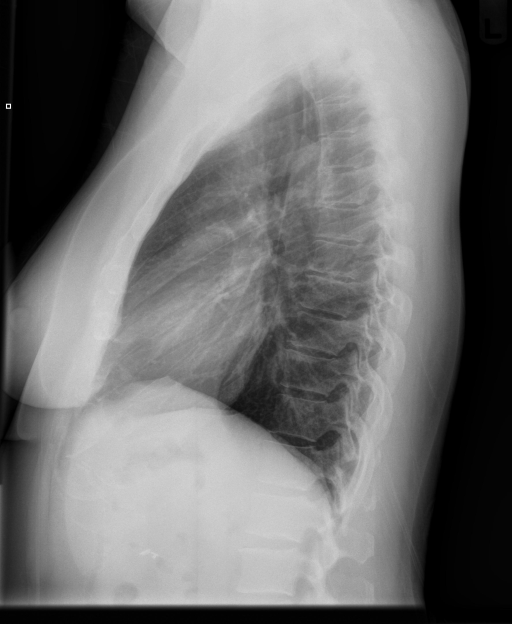
\includegraphics[width=4cm]{AppendixA/AppendixAFigs/originales/laterales/imagen10.png}}
%         \subfigure[][\label{fig:imgtl11} $SSIM = 1$ \newline $LTG = 1$ \newline $\mathscr{H} = 6.2748$ \newline $\mathscr E = 2.4087$
%         ]{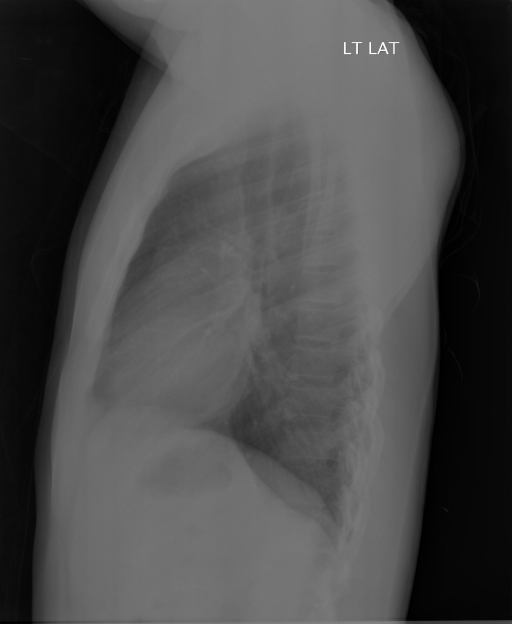
\includegraphics[width=4cm]{AppendixA/AppendixAFigs/originales/laterales/imagen11.png}}
%     \end{center}
%     \label{fig:gral8}
% \end{figure}

% \begin{figure}[H]
%     \begin{center}
%         \subfigure[][\label{fig:imgtl3} $SSIM = 1$ \newline $LTG = 1$ \newline $\mathscr{H} = 5.7765$ \newline $\mathscr E = 2.4201$
%         ]{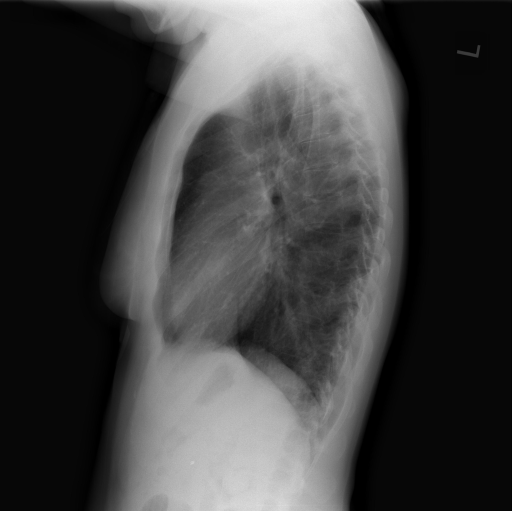
\includegraphics[width=4.5cm]{AppendixA/AppendixAFigs/originales/laterales/imagen3.png}}
%         \subfigure[][\label{fig:imgtl5} $SSIM = 1$ \newline $LTG = 1$ \newline $\mathscr{H} = 6.4335$ \newline $\mathscr E =2.7586$
%         ]{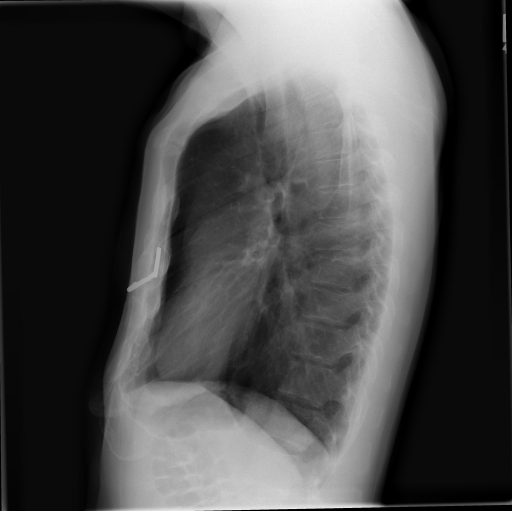
\includegraphics[width=4.5cm]{AppendixA/AppendixAFigs/originales/laterales/imagen5.png}}
%     \end{center}
%     \label{fig:gral9}
% \end{figure}


% \section{Resultado Correlación de Pearson}

% \begin{table}[H]
% \centering
% \caption{Promedio de la correlación de Pearson.}
% \begin{tabular}{|c|c|}
% \hline
% Métricas & Correlación \\
% \hline \hline 
% %-0.9547657122	-0.9866466591	-0.9308066035	-0.9731620476
% $\mathscr{H}$ / \textit{SSIM} & -0.9554 \\ \hline
% $\mathscr{E}$ / \textit{SSIM} & \textbf{-0.9870}\\ \hline
% $\mathscr{H}$ / \textit{LTG} & -0.9319 \\ \hline
% $\mathscr{E}$ / \textit{LTG} & -0.9731 \\ \hline
% \end{tabular}
% \label{tabla:promcorrelacion}
% \centering
% \end{table}

% \section{Resultados Indicador de Hipervolumen}

% \begin{table}[H]
% \centering
% \caption{Hipervolumen de los Frentes Pareto - Tórax Frontal.}
% \begin{tabular}{|c|c|}
% \hline
% Frente Pareto & Valor Hipervolumen {\it yref}: [6,1] \\
% \hline \hline 
% \it{Robusto} &  0.9987\\ \hline
% \it{Tórax Frontal \ref{fig:img1}} & 0.97088 \\ \hline
% \it{Tórax Frontal \ref{fig:img2}} & 1.07444 \\ \hline
% \it{Tórax Frontal \ref{fig:img4}} & 0.94675 \\ \hline
% \it{Tórax Frontal \ref{fig:img3}} & 0.98474 \\ \hline
% \it{Tórax Frontal \ref{fig:img5}} & 1.18447 \\ \hline
% \it{Tórax Frontal \ref{fig:img7}} & 0.89804 \\ \hline
% \it{Tórax Frontal \ref{fig:img6}} & 1.05435 \\ \hline
% \it{Tórax Frontal \ref{fig:img8}} & 0.94021 \\ \hline
% \it{Tórax Frontal \ref{fig:img9}} & 0.79659 \\ \hline
% \it{Tórax Frontal \ref{fig:img10}} & 0.89486 \\ \hline
% \it{Tórax Frontal \ref{fig:img11}} & 0.97175 \\ \hline
% \it{Tórax Frontal \ref{fig:img12}} & 1.08461 \\ \hline
% \it{Tórax Frontal \ref{fig:img13}} & 0.62923 \\ \hline
% \it{Tórax Frontal \ref{fig:img14}} & 0.85066 \\ \hline
% \it{Tórax Frontal \ref{fig:img15}} & 0.90512 \\ \hline
% \end{tabular}
% \label{tabla:hipervolumen-frontal}
% \end{table}

% \begin{table}[H]
% \centering
% \caption{Hipervolumen de los Frentes Pareto - Tórax Lateral.}
% \begin{tabular}{|c|c|}
% \hline
% Frente Pareto & Valor  Hipervolumen {\it yref}: [6,1] \\
% \hline \hline 
% \it{Robusto} &  1.51317\\ \hline
% \it{Tórax Lateral \ref{fig:imgtll}} & 1.29874 \\ \hline
% \it{Tórax Lateral \ref{fig:imgtl2}} & 1.47126 \\ \hline
% \it{Tórax Lateral \ref{fig:imgtl4}} & 1.34961 \\ \hline
% \it{Tórax Lateral \ref{fig:imgtl6}} & 1.77041 \\ \hline
% \it{Tórax Lateral \ref{fig:imgtl7}} & 1.15427 \\ \hline
% \it{Tórax Lateral \ref{fig:imgtl8}} & 1.13405 \\ \hline
% \it{Tórax Lateral \ref{fig:imgtl9}} & 1.02208 \\ \hline
% \it{Tórax Lateral \ref{fig:imgtl10}} & 1.27029 \\ \hline
% \it{Tórax Lateral \ref{fig:imgtl11}} & 1.45903 \\ \hline
% \it{Tórax Lateral \ref{fig:imgtl3}} & 2.45754 \\ \hline
% \it{Tórax Lateral \ref{fig:imgtl5}} & 1.63800 \\ \hline

% \end{tabular}
% \label{tabla:hipervolumen-lateral}
% \end{table}



% % \bigskip












